\setcounter{secnumdepth}{2}
\section{Bảng phân công công việc và cài đặt xv6}
\subsection{Bảng phân công công việc}
Dưới đây là bảng phân công công việc của nhóm:

\centering
\vskip 0.25 cm
\begin{tabular}{|c|c|c|}
	\hline
	Họ và tên & Chức năng đảm nhiệm & Tiến độ hoàn thành\\
	\hline
	Hồ Minh Quang & Lệnh \textbf{pingpong} & 100\%\\
	\hline
	Hồ Minh Quang & Lệnh \textbf{xargs} & 100\%\\
	\hline
	Lê Hoàng Sơn & Lệnh \textbf{primes} & 100\%\\
	\hline
	Lê Hoàng Sơn & Lệnh \textbf{find} & 100\%\\
	\hline
	Hồ Minh Quang & Viết báo cáo cho các lệnh & 100\%\\
	Lê Hoàng Sơn & được đảm nhiệm & 100\%\\
	\hline
\end{tabular}

\justifying
\subsection{Cài đặt xv6}
Các hướng dẫn cài đặt xv6 đã có sẵn trên Lab 6.1810 của MIT \cite{mit-xv6}. Dưới đây là kết quả cài đặt xv6 của nhóm:

\begin{figure}[h!]
	\centering
	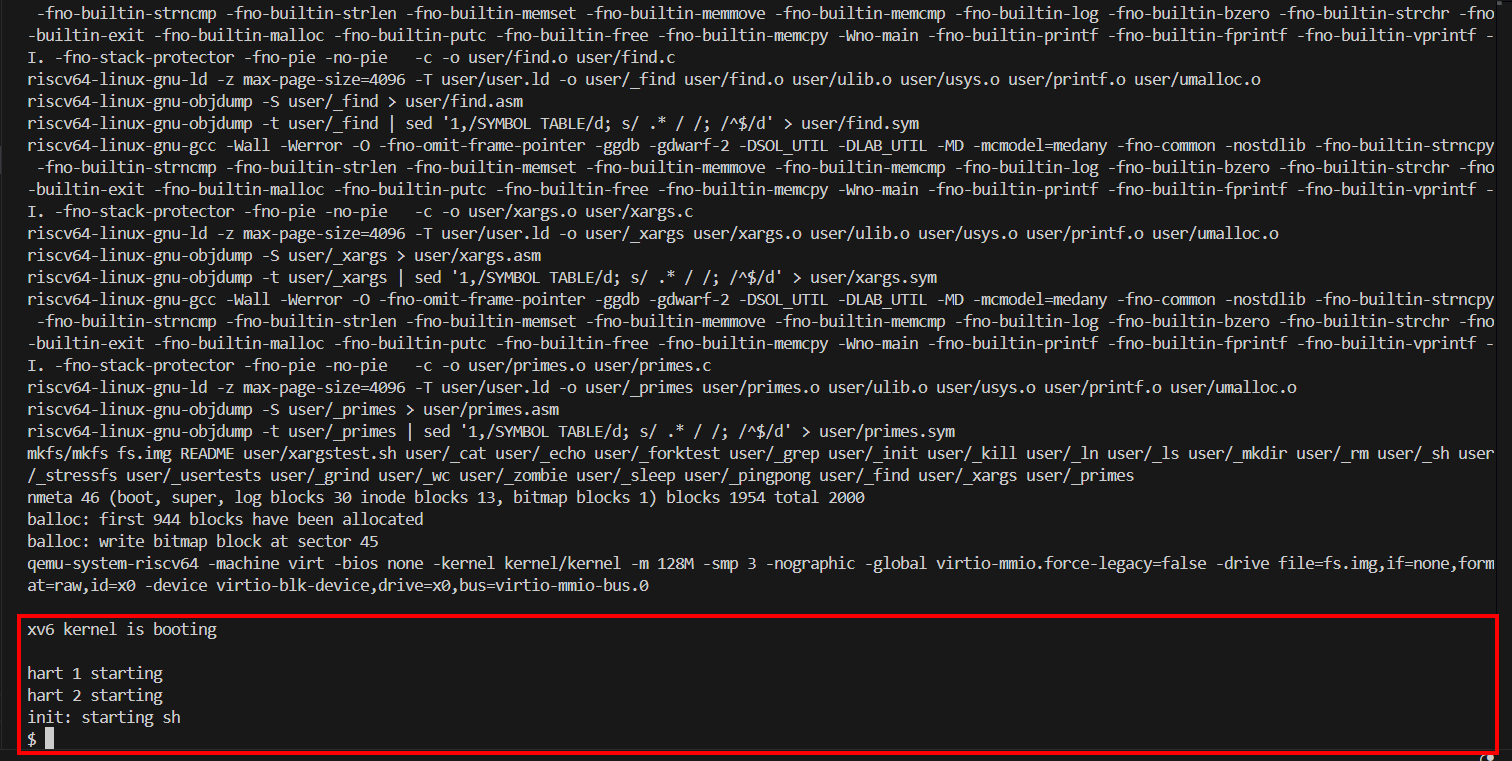
\includegraphics[width=0.9\textwidth]{figures/xv6-launch}
	\caption{Khởi động xv6 trên Linux}
\end{figure}

\justifying
Lệnh \mintinline{shell}|$ git diff origin -- . > 22120295_22120311.patch| được dùng để tạo \linebreak bản vá \verb|diff|.

\subsection{Một số hàm có sẵn trong mã nguồn}
\underline{\mintinline{C++}|int read(int _fd, void* _buffer, int _nbytes)|:} Hàm này được dùng để đọc một số lượng byte trong tập tin \verb|_fd| và lưu vào vùng nhớ con trỏ \verb|_buffer| trỏ tới.

\underline{\mintinline{C++}|int write(int _fd, void* _buffer, int _nbytes)|:} Hàm này được dùng để ghi một số lượng byte vào tập tin \verb|_fd| từ vùng nhớ con trỏ \verb|_buffer| trỏ tới.